%\documentclass[iop]{emulateapj}
\documentclass[aps, pre, onecolumn, nofootinbib, notitlepage, groupedaddress, amsfonts, amssymb, amsmath, longbibliography]{revtex4-1}
\usepackage{tabularx}
\usepackage{graphicx}
\usepackage{hyperref}
\usepackage{xcolor}
\hypersetup{
    colorlinks,
    linkcolor={red!50!black},
    citecolor={blue!50!black},
    urlcolor={blue!80!black}
}
\usepackage{bm}
\usepackage{natbib}
\usepackage{longtable}
\LTcapwidth=0.87\textwidth

\newcommand{\Div}[1]{\ensuremath{\nabla\cdot\left( #1\right)}}
\newcommand{\DivU}{\ensuremath{\nabla\cdot\bm{u}}}
\newcommand{\angles}[1]{\ensuremath{\left\langle #1 \right\rangle}}
\newcommand{\grad}{\ensuremath{\nabla}}
\newcommand{\RB}{Rayleigh-B\'{e}nard }
\newcommand{\stressT}{\ensuremath{\bm{\bar{\bar{\Pi}}}}}
\newcommand{\lilstressT}{\ensuremath{\bm{\bar{\bar{\sigma}}}}}
\newcommand{\nrho}{\ensuremath{n_{\rho}}}
\newcommand{\approptoinn}[2]{\mathrel{\vcenter{
	\offinterlineskip\halign{\hfil$##$\cr
	#1\propto\cr\noalign{\kern2pt}#1\sim\cr\noalign{\kern-2pt}}}}}

\newcommand{\appropto}{\mathpalette\approptoinn\relax}

\newcommand\mnras{{MNRAS}}%

\begin{document}
\author{Evan H. Anders}
\affiliation{Dept. Astrophysical \& Planetary Sciences, University of Colorado -- Boulder, Boulder, CO 80309, USA}
\affiliation{Laboratory for Atmospheric and Space Physics, Boulder, CO 80303, USA}
\author{Benjamin P. Brown}
\affiliation{Dept. Astrophysical \& Planetary Sciences, University of Colorado -- Boulder, Boulder, CO 80309, USA}
\affiliation{Laboratory for Atmospheric and Space Physics, Boulder, CO 80303, USA}
\author{Jeffrey S. Oishi}
\affiliation{Department of Physics and Astronomy, Bates College, Lewiston, ME 04240, USA}
\title{Accelerated convergence of convective simulations using boundary value problems}

\begin{abstract}
We present a method for using coupling Boundary value problems (BVPs) with Initial value problems (IVPs)
in order to achieve thermally converged convective solutions on dynamical timescales, rather than the
long thermal timescale.  We demonstrate the similarity between the solution reached via BVP and the
solution reached by a long thermal rundown of the IVP, and demonstrate that this method works at a
large range of supercriticalities.  We use this method to achieve converged solutions at high Ra,
and discuss its extension to more complex scenarios, such as stratified, compressible convection.
\end{abstract}
\maketitle

\section{Introduction}
\label{sec:intro}
Natural convection occurs in the presence of disparate timescales. Granules on the
solar surface overturn on the order of 10 minutes, whereas deep motions in the Sun are likely at
low Mach number and constrained by the solar rotation rate of $\sim$1 month.  
Both of these dynamical timescales are vastly shorter than the Sun's average timescale of energy transport,
which is the Kelvin-Helmholtz timescale of nearly $3 \times 10^7$ \emph{years} \cite{stix2003}. 
As simulations aim to model natural convection
by increasing into the high-Rayleigh Number (Ra) regime, where diffusive timescales are much
longer than dynamical timescales \cite{Anders&Brown2017}, achieving converged simulations will 
require runs which span a greater number of convective timescales in order to thermally converge.
Furthermore, with increasing Ra and decreasing diffusivities, motions become more turbulent
and require finer grid meshes and shorter timesteps to resolve turbulent motions, increasing the simulation
time required for each overturn timescale.  
These two effects conspire to make achieving thermally converged, high-Ra, astrophysically interesting
simulations an intractable problem using modern numerical tools.

Prior studies of stratified convection in which a convective layer lies between stable layers
have used the knowledge of Mixing Length Theory (MLT) to adjust the initial thermodynamic structure of
the atmosphere to a state which is closer to the adiabat chosen by convection \cite{brandenburg&all2005}.
However, most studies of convection do not contain stable layers above and below the convection
zone, and the presence of hard boundaries and the boundary layers that they form make it difficult to
know the correct evolved adiabat \emph{a priori}.

Here we present a method for using simple boundary value problems (BVPs), 
along with information about the evolved flow fields,
to fast-forward the slow thermal evolution of convecting simulations.  
We run two sets of experiments: one in which we allow convective simulations to evolve for a
full thermal timescale before taking measurements, and another in which we employ a fast-forwarding,
BVP technique which occurs on dynamical timescales. We compare these two sets of simulations to
show the validity of the BVP technique.  Then, we use the BVP technique to run simulations
at high Ra, in the regime where running for thermal timescales becomes computationally intractable.

\section{Experiment}
\label{sec:experiment}
We adopt the Oberbeck-Boussinesq approximation.  Under this choice, the
fluid has constant kinematic viscosity ($\nu$), thermal diffusivity ($\kappa$), and coefficient
of thermal expansion ($\alpha$). The variables of the fluid that are evolved are the velocity,
$\bm{u} = u\hat{x} + v\hat{y} + w\hat{z}$, the temperature $T = T_0 + T_1$, and the pressure.
The density of the fluid is a constant $\rho_0$, except on the
term where the constant gravitational acceleration, $\bm{g} = - g\hat{z}$ acts in the vertical momentum equation, 
in which case it is $\rho = \rho_0(1  - \alpha T_1)$.  
Under these choices, the equations of motion are \cite{spiegel&veronis1960}
\begin{gather}
\DivU = 0, 
	\label{eqn:dim_incompressible}
\\
\frac{\partial \bm{u}}{\partial t} + \bm{u}\cdot\grad\bm{u} =
-\frac{1}{\rho_0}\grad P - g( 1 - \alpha T_1)\hat{z} + \nu\grad^2\bm{u}, 
	\label{eqn:dim_bouss_momentum}
\\
\frac{\partial T_1}{\partial t} + \bm{u}\cdot\grad(T_0 + T_1) = \kappa\grad^2 T_1,
	\label{eqn:dim_bouss_energy}
\end{gather}
We non-dimensionalize these equations such that length scales are in units of the layer height ($L_z$),
temperature is in units of the initial temperature jump across the layer ($\Delta T_0 = L_z \grad T_0$), 
and time is in units of the freefall timescale ($L_z / v_{\text{ff}}$), where the freefall velocity is
$v_{\text{ff}} = \sqrt{\alpha g L_z^2 \grad T_0}$.
We further re-arrange the momentum equation by introducing a reduced pressure
$\varpi \equiv P / \rho_0 + \phi + |\bm{u}|^2 / 2$, where $\bm{g} = -\grad \phi$ is the gravitational potential.
Despite containing a nonlinear $\bm{u}$ component, the nature of $P$ in \RB convection, as a (whatever it's called)
allows us to treat $\varpi$ as a linear unknown, without a need to resolve its different components.
We time evolve the equations in the form,
\begin{gather}
\DivU = 0, 
	\label{eqn:incompressible}
\\
\frac{\partial \bm{u}}{\partial t} + \grad \varpi - T_1\hat{z} + \mathcal{R}\grad\times\bm{\omega} = \bm{u}\times\bm{\omega}
	\label{eqn:bouss_momentum}
\\
\frac{\partial T_1}{\partial t} - \mathcal{P}\grad^2 T_1 + w \frac{\partial T_0}{\partial z} = - \bm{u}\cdot\grad T_1,
	\label{eqn:bouss_energy}
\end{gather}
where $\bm{\omega} = \grad \times \bm{u}$ is the vorticity. We find this form of the momentum equation to
be slightly faster numerically than the standard form in Eq. (\ref{eqn:dim_bouss_momentum}).
The dimensionless control parameters are set by the Rayleigh and Prandtl numbers,
\begin{equation}
\mathcal{R} \equiv \sqrt{\frac{\text{Pr}}{\text{Ra}}}, \qquad \mathcal{P} \equiv \frac{1}{\sqrt{\text{Pr}\,\text{Ra}}}, \qquad
\text{Ra} = \frac{g \alpha L_z^4 \grad T_0}{\nu\chi} = \frac{(L_z\,v_{\text{ff}})^2}{\nu\chi}, \qquad \text{Pr} = \frac{\nu}{\chi}.
\end{equation}
The dimensionless vertical extent of the domain is $z = [-1/2, 1/2]$, and at the boundaries
we impose no-slip, impenetrable boundary conditions such that $w = u = v = 0$ at $z = \pm 1/2$.
At the lower boundary, we employ a fixed flux condition such that $\partial T_1 / \partial z = 0$
at $z = -1/2$, and we impose a fixed temperature condition $T_1 = 0$ at $z = 1/2$. Both
horizontal directions are periodic, extending over a range $x, y = [0, \Gamma]$, where
the aspect ratio is $\Gamma = 2$.

The chosen thermal boundary conditions at the upper and lower plates
determine key quantities of the evolved state.
Studies of incompressible, Boussinesq, \RB convection often
employ fixed temperature (Dirichlet) or fixed heat flux
(Neumann) boundary conditions at both plates.  
Dirichlet conditions represent plates of infinite conductivity,
whereas Neumann conditions model plates of finite conductivity.  
In both cases, choosing symmetric boundary conditions maintains overall system symmetry, 
and despite evolving towards different thermal structures, both types of conditions
transport heat in the same manner \cite{johnston&doering2009}.
Studies of convection which aim to model
astrophysical systems such as stars often employ a mixture of these
two types of boundary conditions \cite{hurlburt&all1984, cattaneo&all1991, korre&all2017}.  
The flux at the lower boundary is fixed, modeling
the constant energy generation of the stellar core, 
while the outer boundary condition is held at a fixed temperature,
modeling the surface of a star which must output the energy generated internally.
This setup is a useful model for understanding natural
systems, but simulations which employ these boundary conditions suffer from a long 
thermal relaxation as the atmosphere loses energy and approaches the adiabat chosen by the
Dirichlet condition.  We choose these conditions in part to better understand them, and in
part because these conditions minimize the number of assumptions that must be made in
setting up the boundary value problem.

\subsection{The Boundary Value Problem}
\begin{figure}[t]
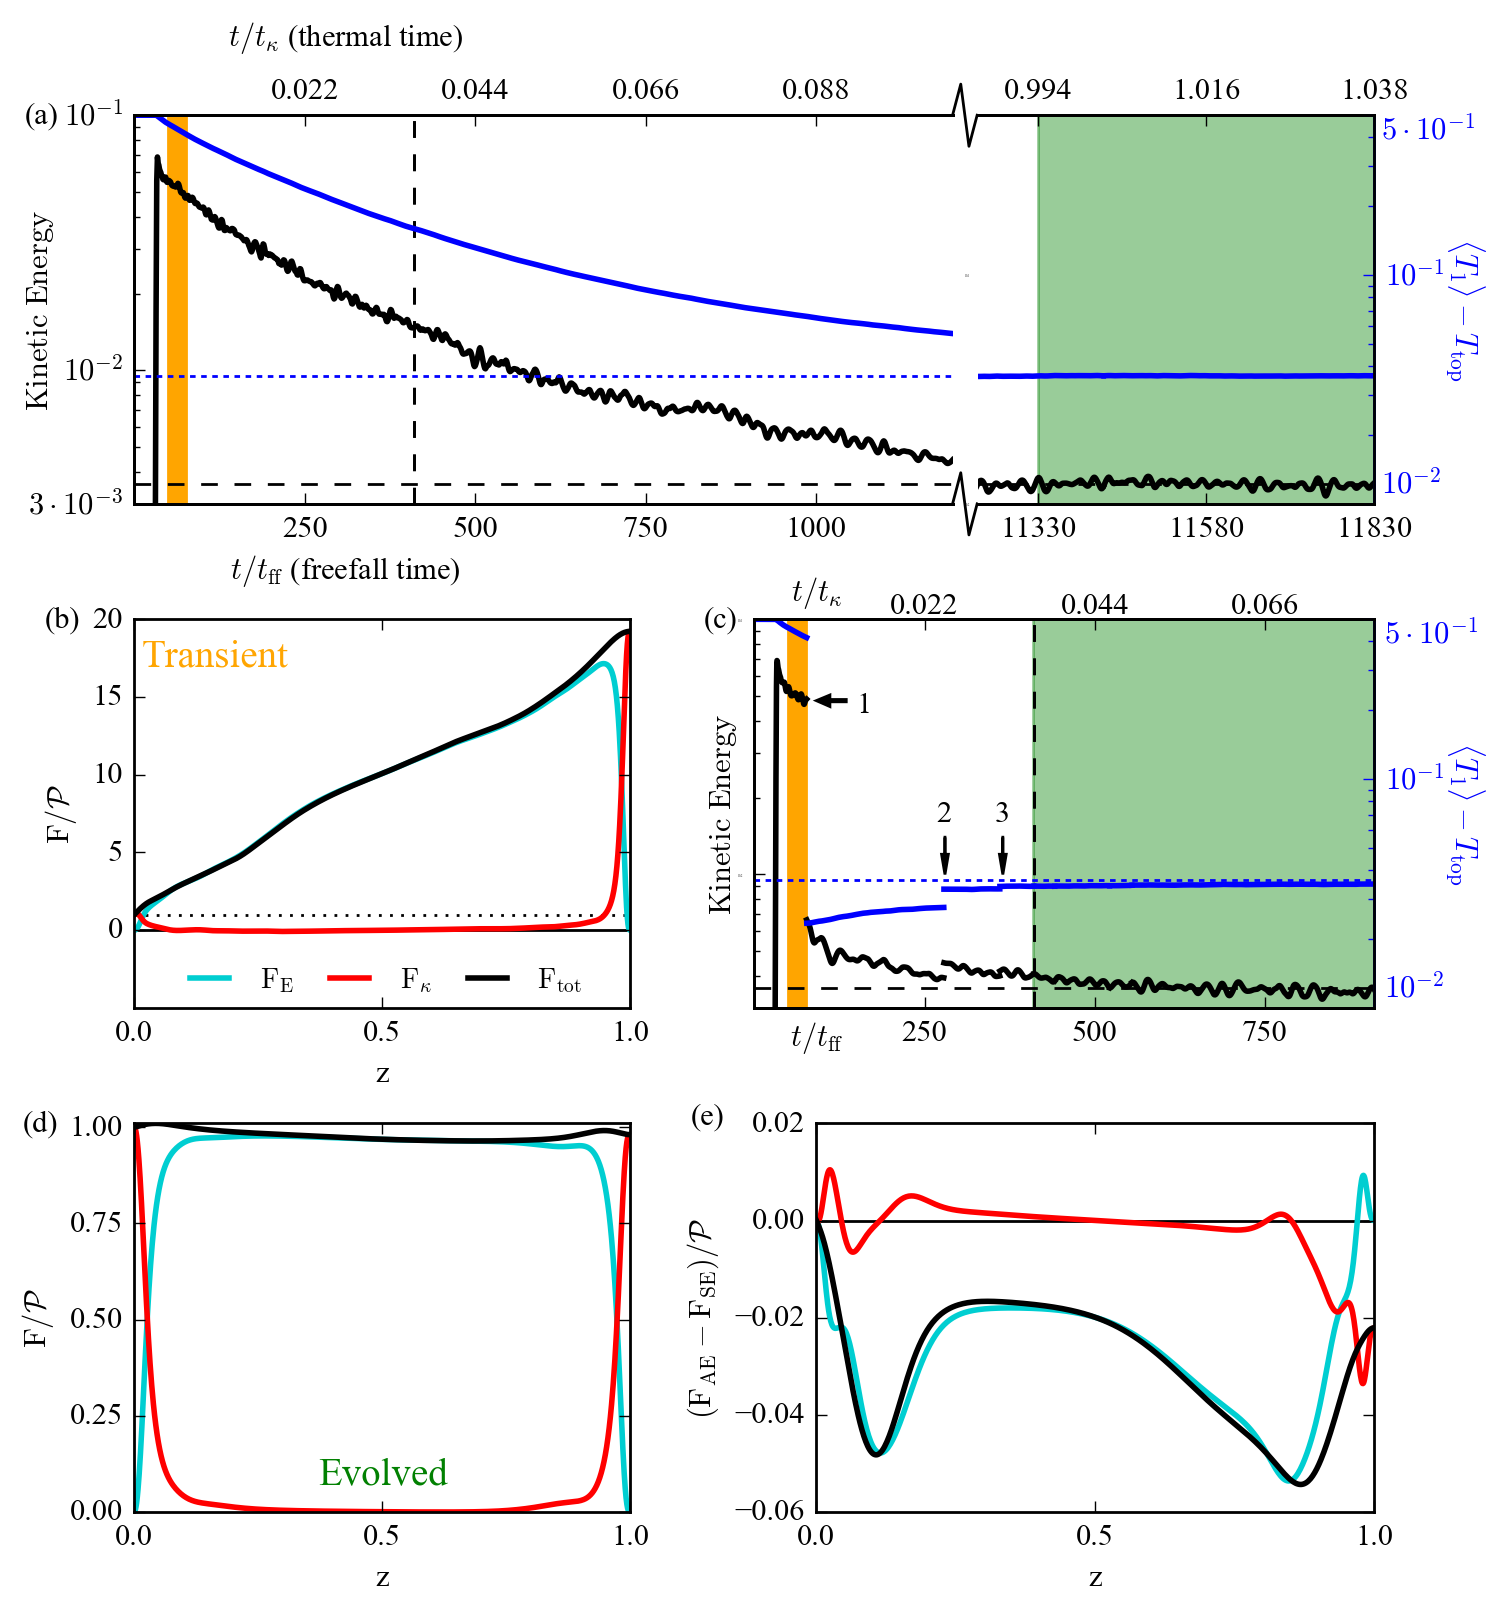
\includegraphics[width=\textwidth]{./figs/time_trace.png}
\caption{Traces of system energies vs. time for a long thermal rundown (a) and BVP convergence
(b) are shown for Ra = $1.30 \cdot 10^8$ ($S = 10^5$).  The horizontal extent of the subplots is set
such that one simulation time unit takes up an equal amount of paper space in (a) and (b).
The dashed vertical line on (a) represents the time at which the BVP is solved on the run in (b),
and the horizontal dashed lines show the equilibrium value of the energies.
(c) System fluxes early in the run (the orange highlights in (a)).  Black is the sum of the flux, purple
is the convective flux, and red is the conductive flux.
(d) Fluxes in the converged rundown IVP compared to the ``converged'' BVP.  The sum of flux is shown in
black \& grey, the convective flux is shown in purple \& pink, and the conductive flux is shown in red \& orange.
(e) The differences between the BVP and rundown fluxes is shown.  While not in perfect agreement, the BVP fluxes
are much closer to the converged state than the initial fluxes, as in (c).
\label{fig:time_trace} }
\end{figure}

It is a reasonable assumption to naively guess that convection will evolve the mean temperature profile that
drives it over the course of a thermal diffusion time, $t_\chi \approx \mathcal{P}^{-1}$. Thus, as Ra
increases, the timescale for achieving a thermally converged mean temperature profile becomes intractable.
This prohibitively long thermal timescale in a Direct Numerical Simulation (DNS) 
can be skipped by coupling the DNS with a simple Boundary Value Problem
(BVP) solve. By using information about the evolved dynamical state of the atmosphere,
a BVP can be used to solve for the evolved atmospheric state on short timescales.
A comparison of a simulation running for the thermal timescale, and another where a BVP is used
to fast-forward atmospheric evolution, are shown in Fig \ref{fig:time_trace}a\&b.

The Boussinesq BVP in essence contains equations of hydrostatic balance and thermal equilibrium,
\begin{gather}
\frac{\partial}{\partial z}\angles{\varpi} - \angles{T_1}\hat{z} = \angles{\bm{u}\times\bm{\omega}},
	\label{eqn:bouss_BVP_momentum}
\\
\frac{\partial}{\partial z}\angles{wT_1} - \frac{1}{\text{Pr}\text{Ra}}\frac{\partial^2}{\partial z^2} \angles{T_1} = 0,
	\label{eqn:bouss_BVP_energy}
\end{gather}
where $\angles{A}$ represents a time- and horizontally averaged profile of the quantity $A$.  
These
equations arise from assuming that the atmosphere is in a steady state ($\partial_t \rightarrow 0$),
then taking time and horizontal averages of Eqns (\ref{eqn:bouss_momentum}\&\ref{eqn:bouss_energy}) and
neglecting terms that vanish due to the symmetry of the problem.
Convective flows
are perturbations around a thermal profile defined by these equations in the proper evolved, statistically stationary state.

Under eqns (\ref{eqn:bouss_BVP_momentum}\&\ref{eqn:bouss_BVP_energy}), 
the thermal structure ($\angles{T_1}$, $\angles{\varpi}$) of the atmosphere is fully determined by the specification
of two profiles: the convective flux, $F_{conv} = \angles{w T_1}$, and the nonlinear advection, $\angles{\bm{u}\times\bm{\omega}}$.  
If these profiles are known, then 
solving for $\angles{T_1}$ and
$\angles{\varpi}$ depends only upon the choice of boundary conditions.

By definition, the profile of $F_{conv}$ is not in its time stationary early in the DNS.  
In fact, as the atmosphere approaches the
isotherm specified by the upper (fixed $T$) boundary condition, the motions display an asymmetric flux as energy
leaks through the upper boundary condition (Fig. \ref{fig:time_trace}c) in order to reach a lower temperature state.
In order to construct the evolved convective flux from the current fluxes in the atmosphere,
we assume that the atmospheric dynamics have properly developed the thickness of the boundary layers, 
or that the quantities
\begin{equation}
f_{\text{conv}} = \frac{F_{\text{conv}}}{F_{\text{tot}}}\qquad
f_{\text{cond}} = \frac{F_{\text{cond}}}{F_{\text{tot}}}
\end{equation}
early in the evolution are the same as those in the final steady state solution. By definition, the
evolved total flux through the atmosphere must be the same as the flux entering the atmosphere at the
bottom boundary, $F_{\text{tot, steady}} = F_{\text{bot}}$.  The proper enthalpy flux profile to feed in
to Eqn. (\ref{eqn:bouss_BVP_energy}) is then 
$\angles{w T_1}_{\text{steady}} = F_{\text{tot, steady}} \cdot f_{\text{conv}}$.  Presumably, over the
course of the simulation, the velocity field and temperature fluctuations naturally scale like
$d(z) = \angles{w T_1}_{\text{steady}}/\angles{w T_1}$, and so it is necessary to multiply the velocity
field and the fluctuations around the mean in $T_1$ by $\sqrt{d}$.  This also means that
$\angles{\bm{u}\times\bm{\omega}}_{\text{steady}} = d \angles{\bm{u}\times\bm{\omega}}$. Once these profiles
are appropriately adjusted, they can be used in the BVP solve to find the mean profiles of $T$ and $\varpi$.

In general, the BVP solve is completed in the following steps:
\begin{enumerate}
\item Run the convective DNS. Once the convection achieves a volume-averaged Re of $\sqrt{\text{Ra}/\text{Ra}_{\text{crit}}}$,
wait for 50 time units.  Then, start taking the averages of $F_{\text{conv}}$ and $F_{\text{tot}}$, waiting either
30 time units or until the profiles are converged to 1 part in 1000, whichever is a more difficult. This ensures that
the profiles being used in the BVP are steady and smooth, and that they sample the full behavior of the convection.
\item Construct $\angles{w T_1}_{\text{steady}}$ and $\angles{\bm{u}\times\bm{\omega}}_{\text{steady}}$
from the flux profiles.
\item Solve for $\angles{T_1}$ and \angles{\varpi} of the
evolved state.  Adjust the mean profiles in the IVP.
\item Multiply the velocity field and the fluctuations in $T_1$ about its horizontal average by $\sqrt{d}$ in the IVP. 
\item Continue running the IVP for 50 time units to allow for the velocities to equilibrate to their new background state.
\end{enumerate}

\subsection{Numerics}
We utilize the 
Dedalus\footnote{\url{http://dedalus-project.org/}} 
pseudospectral framework \cite{burns&all2016} to time-evolve  
(\ref{eqn:incompressible})-(\ref{eqn:bouss_energy}) 
using an implicit-explicit (IMEX), third-order, four-step 
Runge-Kutta timestepping scheme RK443 \cite{ascher&all1997}.  
The temperature field is decomposed as $T = T_0(z) + T_1(x, y, z, t)$
and the velocity is $\bm{u} = w\bm{\hat{z}} + u\bm{\hat{x}} + v\bm{\hat{y}}$.
In our 2D runs, $v = 0$.
Variables are time-evolved on a dealiased Chebyshev (vertical)
and Fourier (horizontal, periodic) domain in which the
physical grid dimensions are 3/2 the size of the coefficient grid.  
Domain sizes range from
32x128 coefficients at the lowest values of 
Ra to 1024x4096 coefficients at Ra $> 10^{9}$ in 2D.

As initial conditions, we fill $T_1$ with
random white noise whose magnitude is $10^{-6}(\text{Ra Pr})^{-1/2}$.
This ensures that the initial perturbations are much smaller than the
evolved convective temperature perturbations, even at large Ra.
We filter this noise spectrum in coefficient space, 
such that only the lower 25\% of the coefficients
have power.

In 2D, there are often multiple steady state solutions (e.g., 2-roll and 3-roll
solutions) which have slightly different flow properties (heat transport, etc.).
Even though the initial perturbations are very small, they shape the convective
transient and thus determine the nature of the steady state convection, at least in
the laminar regime.  In order to ensure that our results are not biased by differences
in flow structure, we ran the simulations using distinct random temperature perturbations
so as to compare statistics in comparable flow fields.  In 3D, rolls are nonstationary over
convective timescales, and so these effects need not be considered there.

\section{Results}
While the differences in the fluxes in Fig. \ref{fig:time_trace} are small, it is important
to determine if the velocity fluctuations and point-by-point nonlinear transport are the same
in the evolved state.  Fig. \ref{fig:pdf_comparison} overlays the probability distribution functions
of the vertical and horizontal velocities, as well as the fully nonlinear portion of the convective
flux for the same case as is shown in Fig. \ref{fig:time_trace}.  The PDFs are quite similar visually,
and have a similarity of (XYZ) according to a Kolmogorov-Smirnov statistic.

In addition to getting the nonlinear dynamics mostly correct, we show that the BVP method retrieves the
proper temperature profile, see e.g., Fig. \ref{fig:temp_comparison}.  Here the BVP profile retrieves the
mean profile of the temperature to within 1\% accuracy, and temperature fluctuations in the two runs
have a similarity of (XYZ) according to a Kolmogorov-Smirnov statistic.

This method works across a broad range of supercriticality.  In Fig. \ref{fig:parameter_space_comparison},
we show measurements of the volume-averaged Nusselt number, Reynolds number, and temperature.
We use standard definitions of the Nusselt number and Reynolds numbers,
\begin{equation}
\text{Nu} = \frac{\angles{wT - (\text{Ra Pr})^{-1/2}\grad T}}{\angles{- (\text{Ra Pr})^{-1/2} \grad T}} =
1 + \frac{\angles{wT}}{-\Delta T}\sqrt{\text{Ra Pr}}, \qquad \text{Re} = \frac{|\bm{u}| L_z}{\nu},
\end{equation}
where $\Delta T = T(z = 1/2) - T(z = -1/2)$ is the evolved temperature difference
between the top and bottom plates.  This form of the Nusselt number is valid even when
the system is not yet in flux equilibrium, and reduces to the standard fixed flux definition
of Nu  = $[1 - \angles{wT} / P]^{-1}$ \cite{johnston&doering2009}. We find a scaling law of
Nu $\propto \text{Ra}^{2/3}$, much steeper than a standard 2/7 or 1/3 scaling law
\cite{johnston&doering2009}. Furthermore, we find that Re$\propto \text{Ra}^{0.425}$. The average temperature
approaches the value at the top of the domain as Ra increases.  

The final morphology of the flows is very important in determining the exact value of Nu and Re.  In general,
a two-roll state vs. a three-roll state will have entirely different statistics -- different Nu, Re, and average
temprature (and as a result, different size boundary layers).  Thus, in 2D studies, it is essential to study flows
of a similar morphology in order to see a clear trend. 

\begin{figure}[t]
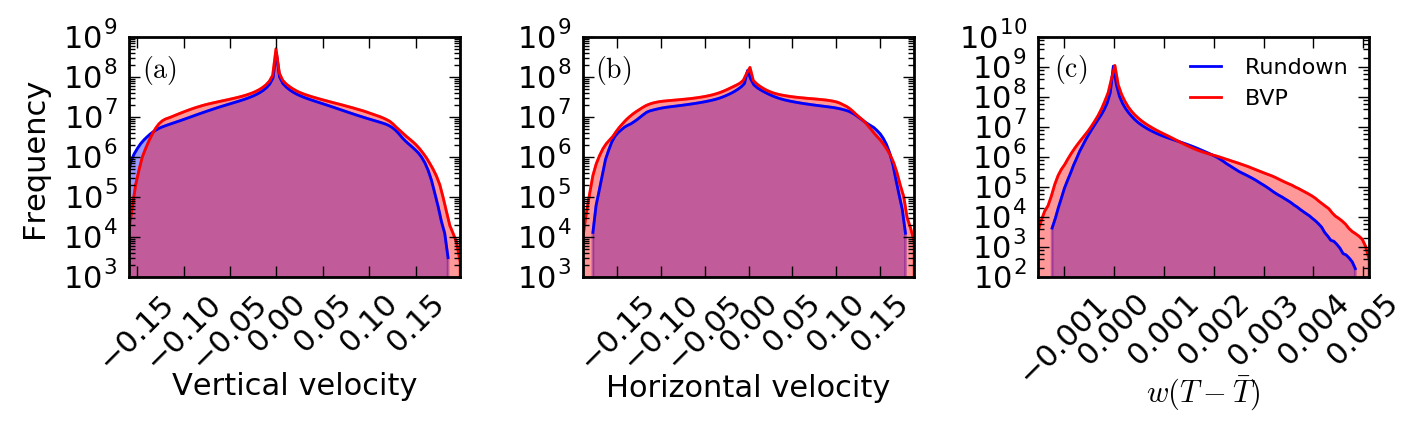
\includegraphics[width=\textwidth]{./figs/pdf_comparison.png}
\caption{Frequency distribution functions of the vertical velocity (a), horizontal velocity (b), and nonlinear
vertical transport (c) are shown for a 2D run at $S = 10^5$.  We sample flows every 0.1 time units for 500 freefall
times, and include the flows at all points on the grid at each of these samples in these distributions.  All
distributions are biased by the no-slip, impenetrable boundary conditions, coupled with the dense spacing of our
Chebyshev grids near the boundaries, so there is a large peak around zero. The distributions, and thus the nonlinear
dynamics, are broadly similar, but they do not pass a two-tailed Kolmogorov-Smirnov similarity test. (NOTE TO
CO-AUTHORS: I NEED TO THINK BETTER ON HOW TO COMPARE PDFS, IF YOU HAVE IDEAS PLEASE SEND THEM)
\label{fig:pdf_comparison} }
\end{figure}

\begin{figure}[t]
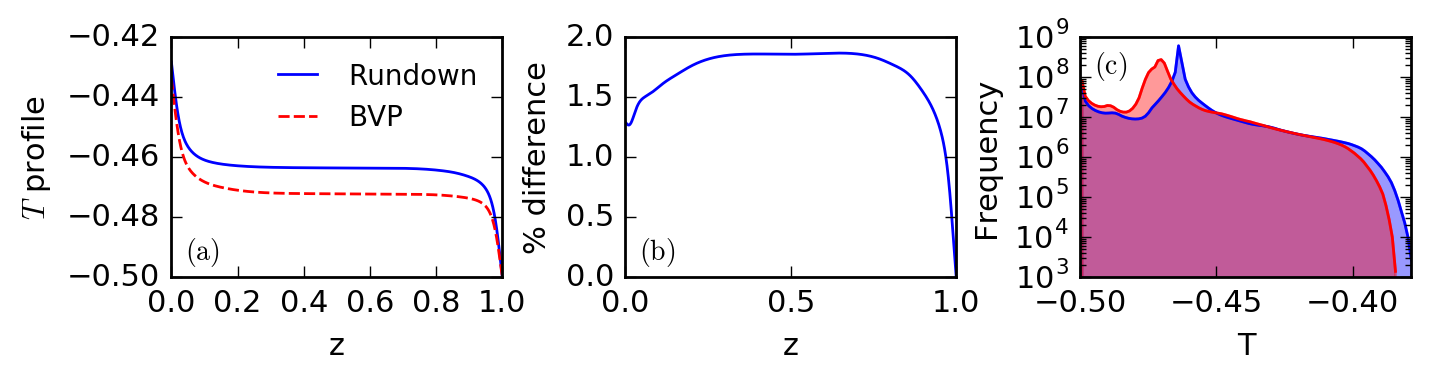
\includegraphics[width=\textwidth]{./figs/temp_comparison.png}
\caption{Comparisons of the evolved thermodynamic states of a BVP solution and a long IVP rundown at
$S = 10^5$ are shown.  (a) Evolved temperature profiles, as a function of height.
(b) The percentage difference between the temperature profiles (as shown in (a)), as a function of height.
(c) Frequency distributions, as in Fig. \ref{fig:pdf_comparison},
comparing the values of the point-by-point temperatures over the averaging
window. The mode of the frequency distribution has a distinct offset between the two runs due to
the clear difference between the profiles in (a), but the
thermal fluctuations about the mean which drive the convection are similar (AS IN FIG. \ref{fig:pdf_comparison},
I NEED TO THINK MORE ON THE PDF COMPARISON).
\label{fig:temp_comparison} }
\end{figure}

\begin{figure}[t]
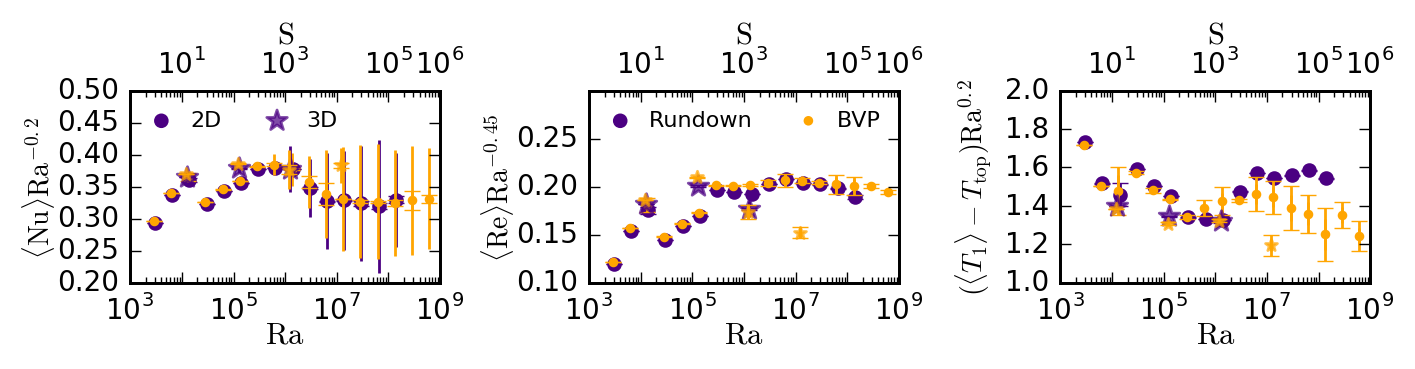
\includegraphics[width=\textwidth]{./figs/parameter_space_comparison.png}
\caption{Compensated scaling plots are shown for the Nusselt number (a), the
Reynolds number (b), and the volume-averaged temperature (c).  All plots are linear(y)-log(x),
and any differences vertically are generally small.  Symbols represent the mean value of
a measurement, vertical lines represent the standard deviation of the measurement over the
time window, and error bars represent the shift in the mean value over the window.
(a) Nu, which measures heat transport, scales roughly like $Ra^{1/5}$, and above Ra$\geq 10^6$,
simulations display horizontally oscillating plumes which have oscillating periods of high transport
and low transport.  The mean value is marginally diminished as a result, and the range of Nu over time
is large. (b) Re, which measures the level of turbulence in the evolved solution, scales as
Ra$^{0.45}$ in 2D and (something else) in 3D. (c) The average temperature flucutation, minus the top
temperature, gives us a measure of the extent of the upper boundary, and is in some ways a more stationary
proxy for Nu, and it displays similar scaling.  The temperature profile is slow to adjust, and differences between
BVP solutions and rundown solutions are easier to pick out.
\label{fig:parameter_space_comparison} }
\end{figure}



\section{Discussion \& Conclusions}
\label{sec:results}
While imperfect, the method presented here is a first step towards taking meaningful measurements
of highly turbulent convection on manageable, human timescales.  As demonstrated in Figs.
1-4, this BVP method quickly converges simulations to within a few percent of the true final
state, while preserving the natural behavior of the convective solution (such as the oscillatory
nature of high-Ra 2D states in \ref{fig:parameter_space_comparison}).  

While not perfect, the BVP method here has one major benefit over some of the other methods
currently being used to achieve high Ra solutions.  One oft-used method is that of bootstrapping,
in which the converged solution of a low-Ra state is used as initial conditions for a higher-Ra
simulation.  While these methods are extremely powerful, they are influenced by hysteresis effects,
and the powerful, steady rolls achieved at low Ra can result in an artifically over-stable high-Ra
roll solution.  The BVP method can be used with random noise initial conditions which allow the
convective solution to be naturally chosen by the dynamics.

One benefit of the method presented here is that it can be easily extended to more complicated
configurations.  For example, to use this method in simulations of stratified compressible convection,
one need only adapt the BVP equations to the appropriate equations of hydrostatic equilibrium,
$\grad P = -\rho \bm{g}$, and thermal equilibrium, $\Div{F_{\text{cond}} + F_{\text{conv}}} = \text{sources}$,
for the problem at hand.  In compressible convection, where the density is allowed to change,
one must also use the knowledge of stellar structure codes and add an equation of mass conservation
in order to ensure that the BVP does not spuriously add or remove mass from the system.

This method can be extended to other boundary conditions, as well.  To solve for fixed temperature
boundary conditions, the difficulty is in finding the amount of flux through the system -- but
this can be done by using the ratios $f_{\text{conv}}$ and $f_{\text{cond}}$.  In the case of
fixed flux boundary conditions, there is degeneracy in the temperature solution which can come
out of the BVP, but in using knowledge about the system -- such as the initial symmetry of the
RB state around $T_1 = 0$, the final solution can be pegged onto the proper profile.




\begin{acknowledgments}
EHA acknowledges the support of the University of Colorado's George 
Ellery Hale Graduate Student Fellowship.
This work was additionally supported by  NASA LWS grant number NNX16AC92G.  
Computations were conducted 
with support by the NASA High End Computing (HEC) Program through the NASA 
Advanced Supercomputing (NAS) Division at Ames Research Center on Pleiades
with allocations GID s1647 and GID g26133.
\end{acknowledgments}


\appendix
\section{Table of Runs}
\begin{center}
\begin{tabularx}{\textwidth}{ X X X X X X X }
\hline													
Ra	&	Supercriticality	&	nz	&	nx	&	$t_{\text{therm}}$	&	$t_{\text{post BVP}}$	&	$t_{\text{avg}}$	\\[1ex]
\hline		\hline											
$2.79 \cdot 10^3$	&	$10^{1/3}$	&	32	&	128	&	$52.8$	&	50	&	100	\\
$6.01 \cdot 10^3$	&	$10^{2/3}$	&	32	&	128	&	$77.6$	&	50	&	100	\\
$1.30 \cdot 10^4$	&	$10^1$	&	32	&	128	&	$114$	&	50	&	100	\\
$2.79 \cdot 10^4$	&	$10^{1 + 1/3}$	&	32	&	128	&	$167$	&	50	&	100	\\
$6.01 \cdot 10^4$	&	$10^{1 + 2/3}$	&	32	&	128	&	$245$	&	50	&	100	\\
$1.30 \cdot 10^5$	&	$10^2$	&	64	&	256	&	$360$	&	100	&	100	\\
$2.79 \cdot 10^5$	&	$10^{2 + 1/3}$	&	64	&	256	&	$528$	&	100	&	100	\\
$6.01 \cdot 10^5$	&	$10^{2 + 2/3}$	&	64	&	256	&	$776$	&	100	&	100	\\
$1.30 \cdot 10^6$	&	$10^3$	&	128	&	512	&	$1.14 \cdot 10^3$	&	100	&	200	\\
$2.79 \cdot 10^6$	&	$10^{3 + 1/3}$	&	128	&	512	&	$1.67 \cdot 10^3$	&	200	&	200	\\
$6.01 \cdot 10^6$	&	$10^{3 + 2/3}$	&	256	&	1024	&	$2.45 \cdot 10^3$	&	200	&	200	\\
$1.30 \cdot 10^7$	&	$10^4$	&	256	&	1024	&	$3.60 \cdot 10^3$	&	200	&	200	\\
$2.79 \cdot 10^7$	&	$10^{4 + 1/3}$	&	256	&	1024	&	$5.28 \cdot 10^3$	&	200	&	200	\\
$6.01 \cdot 10^7$	&	$10^{4 + 2/3}$	&	256	&	1024	&	$7.76 \cdot 10^3$	&	200	&	200	\\
$1.30 \cdot 10^8$	&	$10^5$	&	512	&	2048	&	$1.14 \cdot 10^4$	&	500	&	500	\\
$2.79 \cdot 10^8$	&	$10^{5 + 1/3}$	&	512	&	2048	&	$1.67 \cdot 10^4$	&	500	&	500	\\
$6.01 \cdot 10^8$	&	$10^{5 + 2/3}$	&	512	&	2048	&	$2.45 \cdot 10^4$	&	500	&	500	\\
$1.30 \cdot 10^9$	&	$10^6$	&	1024	&	4096	&	$3.60 \cdot 10^4$	&	500	&	500	\\
\hline													
\end{tabularx}
\end{center}



\bibliography{biblio.bib}
\end{document}
